\chapter{De l’évolution des paysages \acrshort{cis}-régulateurs à l’évolution phénotypique : étude de la perte convergente du phallus chez les oiseaux}
{\hypersetup{linkcolor=GREYDARK}\minitoc}
\label{chap:4-evolpheno}

\section{Introduction}

Les adaptations morphologiques se mettent généralement en place durant le développement embryonnaire des individus et font intervenir des gènes contrôlant la différenciation cellulaire, la croissance et la régionalisation des différentes parties du corps. Ces gènes sont impliqués dans de nombreux processus biologiques et sont alors hautement pléiotropiques, ce qui contraint l’évolution de leur séquence codante. Les mutations qui affectent la séquence protéique codée par ces gènes ont souvent de larges conséquences et sont donc délétères pour l’organisme. Il est ainsi théoriquement attendu que la part des mutations dans les séquences codantes soit bien plus faible que celle des mutations dans les séquences non-codantes pour expliquer des changements morphologiques majeurs impliquant de tels gènes pléiotropes \citep{wray_evolutionary_2007, carroll_evo-devo_2008}. Des variations temporelles ou spatiales de l’expression des gènes seraient en mesure d’expliquer une part importante des changements évolutifs de la morphologie. Par exemple, de nombreuses populations isolées d’épinoches présentent une réduction convergente de la ceinture pelvienne \citep{shapiro_genetic_2004}. Ce phénotype est principalement déterminé par l’expression du facteur de transcription \textit{Pitx1}, qui est impliqué dans le développement de nombreuses structures chez les vertébrés et qui est sous forte sélection purifiante. Les variations morphologiques observées chez les épinoches sont probablement le résultat de nombreuses mutations dans des éléments \acrshort{cis}-régulateurs de \textit{Pitx1}, spécifiquement actifs dans ce tissu \citep{chan_adaptive_2010, thompson_novel_2018}. L’évolution des paysages \acrshort{cis}-régulateurs des gènes peut ainsi participer à des changements morphologiques importants. Les approches de génomique comparative combinées avec des annotations fonctionnelles permettent alors d’identifier les déterminants génétiques qui sont associés à l’évolution d’un phénotype. Détecter la présence, l’absence, l’activité et mesurer le taux d’évolution des éléments \acrshort{cis}-régulateurs peut ainsi permettre d’identifier les mécanismes responsables de changement d’expression des gènes à l’origine des variations phénotypiques. \\

Les causes génétiques initiales ayant provoquées un changement phénotypique peuvent être difficiles à identifier, particulièrement lorsque celui-ci est ancien et que les génomes ont pu diverger. Les pertes phénotypiques sont intéressantes de ce point de vue car quelle que soit la mutation initiale, il est attendu d’observer un relâchement des pressions de sélection purifiante sur les séquences impliquées dans le développement et le maintien de ces caractères \citep{hiller_forward_2012, roscito_phenotype_2018}. Si ces séquences ne sont pas pléiotropes, elles deviennent non-fonctionnelles et évoluent alors de façon neutre. La présence d’une accumulation de mutations ou plus généralement du changement de taux d’évolution sur une séquence fournissent ainsi des indices sur son rôle dans le phénotype ancestral. Les cas de convergence évolutive, dans lesquels plusieurs lignées évoluent indépendamment vers des traits similaires, permettent d’étudier la répétabilité d’un processus évolutif \citep{sackton_convergent_2019}. Les lignées ayant perdu de manière convergente un trait phénotypique présentent ainsi une augmentation parallèle de la divergence sur les séquences impliquées dans ce trait par rapport à leur état ancestral. En analysant les taux d’évolution des gènes codants chez les mammifères, il a par exemple été montré que plusieurs gènes codant pour des récepteurs olfactifs présentent une accélération significative spécifique chez les espèces marines où les sens du goût et de l’odorat sont fortement réduits \citep{chikina_hundreds_2016}. En cherchant à comprendre les mécanismes moléculaires à l’origine de la perte convergente du vol chez les oiseaux, Sackton et collaborateurs n’ont quant à eux pas observé de taux d'évolution convergent dans les séquences codantes \citep{sackton_convergent_2019}. Cependant, grâce à des alignements de génomes complets, il est possible d’effectuer des comparaisons des taux d’évolution à l’échelle génomique et ainsi de cibler des régions présentant des patrons d’évolution convergents en tenant compte des relations phylogénétiques entre espèces \citep{hiller_forward_2012,prudent_controlling_2016, partha_robust_2019}. Avec une telle approche, Sackton et collaborateurs ont détecté des accélérations convergentes des séquences de nombreux éléments \acrshort{cis}-régulateurs potentiels présentant des marques de chromatine ouvertes lors du développement des membres antérieurs \citep{sackton_convergent_2019}. De même, en analysant  les séquences non-codantes conservées à l’échelle de 24 espèces de vertébrés, plusieurs milliers de régions ont montré des taux d’évolution accélérés convergents chez les 4 espèces considérées ayant un mode de vie souterrain \citep{roscito_phenotype_2018}. Plusieurs d’entre elles sont situées dans les promoteurs ou proches des gènes liés au développement ou ayant des fonctions relatives aux yeux, ce qui est cohérent avec la forte régression de cet organe chez ces espèces.\\

\begin{figure}[H]
    \centering
    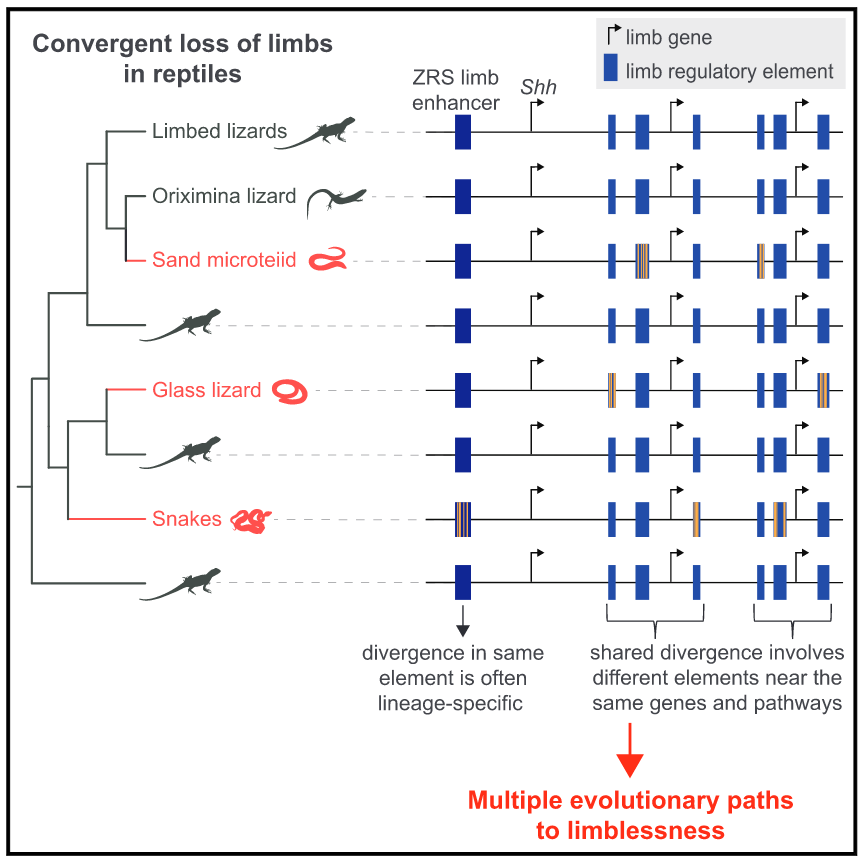
\includegraphics[width=0.7\textwidth, page=1]{figures/IPLOSS/chap4_Fig_intro.png}
    \caption[Évolution des séquences \acrshort{cis}-régulatrices en lien avec la perte convergente des membres chez les reptiles.]{
    \textbf{Évolution des séquences \acrshort{cis}-régulatrices en lien avec la perte convergente des membres chez les reptiles.} Les espèces ayant perdu les membres sont indiquées en rouge dans l'arbre phylogénétique. L'alignement de leurs génomes permet d'analyser l'évolution des séquences \acrshort{cis}-régulatrices (carré bleues) potentiellement impliquées dans la perte phénotypique convergente. Chez les serpents de nombreuses mutations (jaune) dans l'amplificateur ZRS du gène SHH sont impliquées dans cette perte phénotypique. Chez les deux autres espèces de lézard, la séquence de ZRS ne présentent pas de mutations particulières par rapport aux espèces qui possèdent des membres. Les séquences de nombreux autres éléments \acrshort{cis}-régulateurs proches des gènes exprimés normalement dans le développement des membres ont subit une accélération des taux d'évolution chez les espèces ayant perdu les membres. Des éléments \acrshort{cis}-régulateurs différents sont divergents selon les espèces mais sont présent autour des gènes impliqués dans les mêmes voix métaboliques. Tiré de \citep{roscito_convergent_2022}.
    \\
    }
    \label{fig:chap4-fig1}
\end{figure} 

Finalement, il est possible d’identifier si des pressions de sélection partagées ont produit des phénotypes similaires à partir de bases moléculaires identiques, faisant intervenir des mutations similaires sur les mêmes gènes ou éléments régulateurs. Par exemple, peu de séquences présentent une accélération du taux d’évolution convergent entre les serpents et deux espèces de lézards ayant perdu leurs membres (Figure \ref{fig:chap4-fig1}) \citep{roscito_convergent_2022}. La divergence d’éléments \acrshort{cis}-régulateurs distincts auraient impacté les patrons d’expression de gènes impliqués à plusieurs étapes dans la voie de signalisation du développement des membres. La potentielle pléiotropie des éléments \acrshort{cis}-régulateurs de ces gènes du développement pourraient maintenir une sélection purifiante suffisante sur leurs séquences pour ne pas observer de lien avec la perte phénotypique. De plus, les deux espèces de lézards semblent avoir perdu leurs membres relativement récemment par rapport aux serpents ce qui pourrait ne pas avoir laissé suffisamment de temps pour observer une divergence de l’ensemble des séquences impliqués dans ce phénotype.

\section{Etude de la perte convergente du phallus chez les oiseaux}
\label{sec:evol-phallus}

Au cours de ma thèse je me suis intéressé à l’évolution convergente du développement du phallus chez les oiseaux. Cet organe est présent chez l’ancêtre des amniotes mais a été réduit ou perdu dans plusieurs lignées d’oiseaux ainsi que chez une espèce de lézard, le tuatara \citep{brennan_independent_2008, sanger_resurrecting_2015}. Chez les oiseaux, au moins cinq événements indépendants de réduction se seraient produits, notamment dans la lignée des Neoaves représentant plus de 97\% de la diversité actuelle \citep{brennan_independent_2008}. Plusieurs hypothèses évolutives non-exclusives ont été avancées pour expliquer ce changement morphologique majeur \citep{briskie_sexual_1997}. Une première, propose que cette perte soit la conséquence d’une sélection sexuelle pour le choix du partenaire mâle. En effet, l’accouplement chez les espèces d’oiseaux ne possédant pas de phallus nécessite une importante coopération de la femelle pour faire interagir les cloaques des deux individus. Le cloaque est l’orifice postérieur qui est chez ces espèces la seule ouverture commune pour les voies reproductives, digestives et urinaires. La seconde hypothèse avance ainsi que la perte du phallus pourrait être lié à une sélection naturelle pour réduire les risques de transmission sexuelle de pathogène qui pourrait être plus élevés lors d’une intromission \citep{briskie_sexual_1997}. Ce mode de reproduction sans phallus permet également une copulation rapide qui pourrait avoir été sélectionnée pour réduire les risques de prédation \citep{wesotowski_reduction_1999}. Les processus développementaux de ce changement phénotypique sont encore mal connus. Chez le poulet, espèce dont les mâles ne possèdent pas de phallus, il a été montré que le tubercule génital (\acrshort{TG}) se développe d’une manière similaire au canard à des stades embryonnaires précoces \citep{herrera_developmental_2013}. A un stade plus avancé, là où le \acrshort{TG} chez le canard continue de se développer pour former un phallus, la croissance du \acrshort{TG} chez le poulet s’arrête avant de subir une mort cellulaire. Ce processus pourrait être la conséquence de changement de patron d’expression de plusieurs gènes et notamment de \textit{BMP4} qui activerait l’apoptose du \acrshort{TG} chez le poulet \citep{herrera_developmental_2013}. Seule l’expression d’une poignée de gène a été analysée en relation avec ce phénotype chez les oiseaux et souvent uniquement de manière qualitative à l’aide d’hybridation \textit{in situ} sans être quantifié au sein de plusieurs espèces. \\

Dans un premier temps, nous avons ainsi étudié les variations des patrons de l’expression de l’ensemble des gènes codants orthologues entre le poulet et le canard au sein de plusieurs stades de développement cruciaux pour la formation du phallus. Pour ce faire nous avons collaboré avec Patrick Tschopp et Maëva Luxey du laboratoire d’évolution de la régulation de l’Université de Bâle en Suisse. Ces derniers ont pu générer des données de transcriptomiques (\acrshort{RNA-seq}) qui nous ont permis d’identifier des gènes différentiellement exprimés entre les stades et les espèces. Deuxièmement, afin d’identifier les déterminants des variations de l’expression des gènes, nos collaborateurs ont également produit des données d’épigénomiques (\acrshort{ATAC-seq}) indiquant l’accessibilité de la chromatine dans ces mêmes tissus et donc les potentiels éléments \acrshort{cis}-régulateurs. Nous avons analysé la présence et la divergence des séquences de ces éléments entre le canard et le poulet mais aussi la conservation de leur accessibilité entre les tissus. Finalement, nous avons analysé les taux d’évolution de ces éléments au sein de plusieurs lignées d’oiseaux dans le but d’évaluer leur corrélation avec la présence ou l’absence du phallus. Nous avons pour celà bénéficié des alignements de génomes complets publiés récemment par le consortium Birds 10K \citep{feng_dense_2020}. Afin d’associer les éléments non-codants candidats avec leur gènes cibles, l’objectif initial était d’utiliser des données de conformation de la chromatine (\acrshort{Hi-C}) disponible pour plusieurs échantillons chez le poulet. Cependant pour des contraintes de temps, nous avons pour l’instant utilisé une approche classique de voisinage. \\

L’ensemble de ce travail n’est pas encore complètement finalisé, la partie qui suit n’est ainsi que l’ébauche d’un article à partir des résultats que nous commençons à comprendre. Par la suite, nous avons par exemple prévu d’analyser les données de \acrshort{Hi-C} disponibles pour le poulet pour décrire les paysages \acrshort{cis}-régulateurs des gènes candidats. Nous comptons également évaluer l’implication de l’évolution des séquences codantes dans l’évolution de ce phénotype. Notamment, nous souhaitons analyser l’évolution du répertoire des gènes ainsi que la divergence des séquences protéiques au sein des génomes d’oiseaux étudiés pour potentiellement détecter des traces d’accélération du taux d’évolution ou de sélection positive. Grâce à PELICAN, un outil développé par des collègues au LBBE, nous avons également prévu d’analyser la convergence des profils d’acides aminés sur les séquences protéiques.\\

Finalement, dans le cadre de ce projet nous avons également séquencé et assemblé le premier génome du hocco à pierre (\textit{Pauxi pauxi}). Il s’agit d’un oiseau de la famille des Cracidés possédant un phallus et ayant une position phylogénétique intéressante pour l’étude de l’évolution de ce phénotype. Nous avons inclus cet oiseau dans les analyses présentées dans l’article suivant mais nous avons souhaité détailler les caractéristiques de son génome, notamment grâce à des annotations en gènes et en éléments répétés, dans un travail présenté en Annexe (cf \ref{annexe:hocco}). Cet oiseau possède également une excroissance osseuse sur le crâne similaire à plusieurs lignées d’oiseaux. A l’aide d’alignement de séquences protéiques et de PELICAN, nous avons mis en évidence des gènes présentant un profil convergent d’acides aminés et pouvant être des candidats intéressants pour expliquer ce phénotype.
